\section{Exercise 1 - Mid-depth temperature and \delO{SW} reconstruction}

\begin{figure}
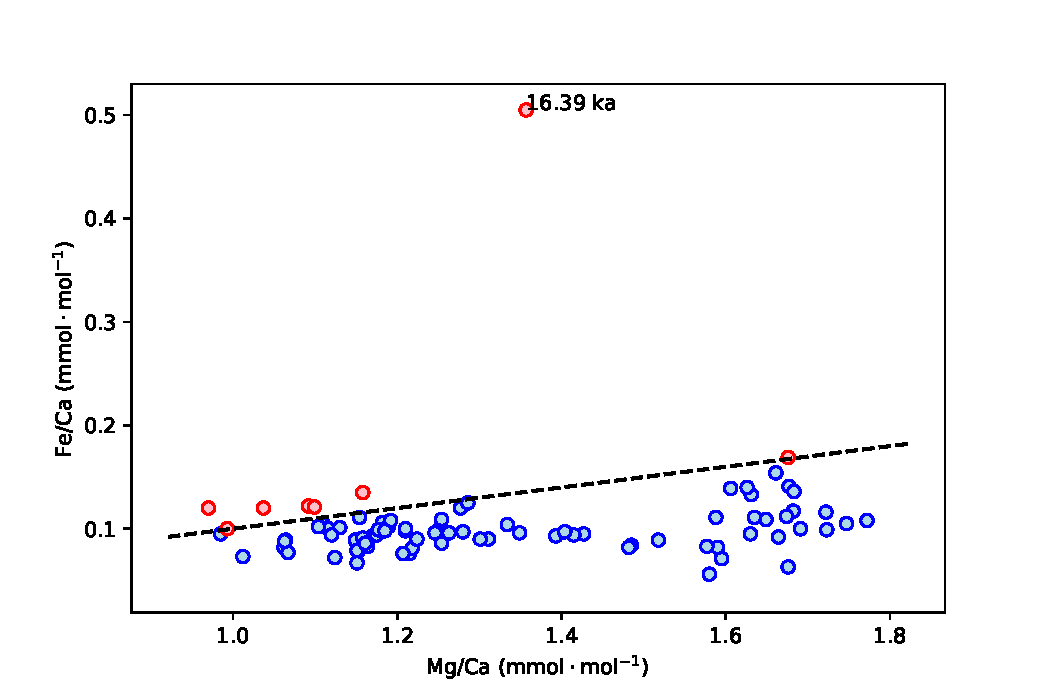
\includegraphics[width=\textwidth]{img/scatter_MgCa_x_FeCa_contaminated.pdf}
    \caption{Scatter plot of bottom water temperature from Mg/Ca palaeothermometry against ice volume corrected oxygen isotope excursion (\delO{SW}), both from benthic foraminifera M. barleeanuum.
             Red points mark potentially contaminated measurements.}
        \label{fig:Mg_Fe}
\end{figure}

\begin{figure}
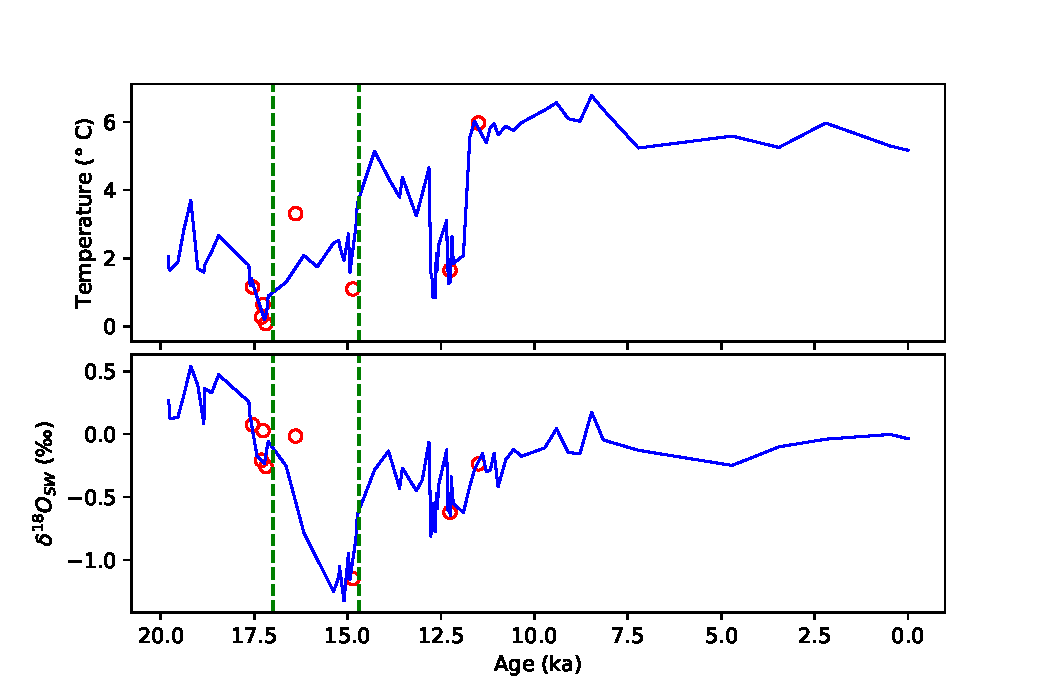
\includegraphics[width=\textwidth]{img/timeseries_temp_and_d18Osw.pdf}
    \caption{Time series of: ice-volume corrected oxygen isotope excursion (top); bottom water temperature (bottom).
             Dashed lines indicate approximate boundaries of Heinrich Stadial 1; red points mark rejected measurements.}
        \label{fig:timeseriestempd18Osw}
\end{figure}

According to \citeauthor{barker2003study}\parencite{barker2003study}, Mg/Ca measurements are determined to be "potentially significantly contaminated" by clay silicates (which can be high in Mg) if the Fe/Mg ratio exceeds 0.1, so measurements here *could* be rejected on the criteria:
$$
\frac{Fe/Mg}{Mg/Ca} > 0.1 \, \mathrm{mol \cdot mol^{-1}}
$$

However, rather apply this criteria naively, it is useful to visually assess the magnitude of possible contamination criteria first.
Of the 8 measurements meeting the criteria are rejected (red circles in Figures \ref{fig:Mg_Fe}, \ref{fig:timeseriestempd18Osw}.
